% ============================================================
% Chapter 19: Problem 18 — Tessellation of Space
% ============================================================

\chapter{Tessellation of Space}

% ------------------------------------------------------------
\begin{figure}[htbp]
\centering
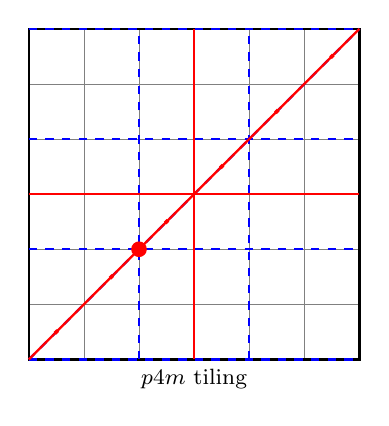
\begin{tikzpicture}[scale=0.7]
  \draw[step=1,gray,very thin] (0,0) grid (6,6);
  \draw[thick] (0,0) -- (6,0) -- (6,6) -- (0,6) -- cycle;
  \draw[thick,blue,dashed] (0,0) -- (6,6);
  \draw[thick,blue,dashed] (2,0) -- (2,6);
  \draw[thick,blue,dashed] (4,0) -- (4,6);
  \draw[thick,blue,dashed] (0,2) -- (6,2);
  \draw[thick,blue,dashed] (0,4) -- (6,4);
  \draw[thick,blue,dashed] (0,0) -- (6,0);
  \draw[thick,blue,dashed] (0,6) -- (6,6);
  \draw[thick,red] (0,0) -- (6,6);
  \draw[thick,red] (2,2) -- (2,2) node[circle,fill,inner sep=2pt]{};
  \foreach \x in {0.5,1.5,2.5,3.5,4.5,5.5}
    \draw[red] (\x,\x) circle (1pt);
  \draw[thick,red] (3,0) -- (3,6);
  \draw[thick,red] (0,3) -- (6,3);
  \node[below] at (3,0) {\footnotesize $p4m$ tiling};
\end{tikzpicture}
\caption{Square tiling with $p4m$ wallpaper group symmetry. Blue dashed lines indicate reflection axes (horizontal, vertical, and diagonal). The pattern has 4-fold rotational symmetry at the corners and centers of squares.}
\label{fig:p4m}
\end{figure}

\section{Historical Context}
% ------------------------------------------------------------

Humans have been fascinated by tilings for millennia. The floor mosaics of ancient Rome, the intricate geometric patterns of Islamic art, and the decorative tilings of the Dutch artist M.\,C.\ Escher all reflect a deep human impulse: to fill the plane---and space---with repeating patterns, endlessly and without gaps.

The mathematical study of tilings begins with a simple question: \emph{can you cover a surface entirely with congruent shapes, with no overlaps and no gaps?} Such a covering is called a \textbf{tessellation} (or, in more modern usage, a \textbf{tiling}).

\subsection{Regular Tessellations of the Plane}

The earliest rigorous result is the classification of \textbf{regular tessellations} of the Euclidean plane $\mathbb{R}^2$. A tessellation is called \textbf{regular} if its tiles are congruent regular polygons, and if the arrangement of tiles around every vertex is the same. Euclid knew---though he did not state it in these terms---that there are exactly \textbf{three} regular tessellations of the plane:

\begin{itemize}
    \item The triangular tiling: equilateral triangles, six meeting at each vertex.
    \item The square tiling: squares, four meeting at each vertex.
    \item The hexagonal tiling: regular hexagons, three meeting at each vertex.
\end{itemize}

The proof is elementary: if $p$-gons tile regularly, then the interior angle $(1-2/p)\pi$ must divide $2\pi$ evenly, so $2p/(p-2)$ must be an integer. The only solutions are $p = 3, 4, 6$.

If we relax the requirement that the tiles be regular polygons but keep the condition that all tiles are congruent and the pattern is periodic, the picture becomes richer. The full classification of \textbf{periodic tilings of the plane}---equivalently, the classification of \textbf{wallpaper groups} or \textbf{plane crystallographic groups}---yields exactly \textbf{17 distinct groups}. This classification was completed by Evgraf Fedorov in 1891, and independently by George Pólya in 1924. These 17 groups exhaust all possible symmetry types of a two-dimensional repeating pattern.

\subsection{Platonic Solids and Regular Polyhedra}

The three-dimensional analogue of a regular polygon is the \textbf{regular polyhedron}. The ancient Greeks knew---and Euclid proved in the \emph{Elements}---that there are exactly \textbf{five} Platonic solids:

\begin{itemize}
    \item The tetrahedron (4 triangular faces),
    \item The cube (6 square faces),
    \item The octahedron (8 triangular faces),
    \item The dodecahedron (12 pentagonal faces),
    \item The icosahedron (20 triangular faces).
\end{itemize}

The proof that there are only five uses the same angle-counting argument as for regular tessellations of the plane: the sum of angles at each vertex must be less than $2\pi$, and the number of faces meeting at each vertex must be an integer. The five Platonic solids are the only solutions.

Kepler, in his \emph{Harmonices Mundi} (1619), extended this classification by considering \textbf{semiregular polyhedra}---solids whose faces are regular polygons but not necessarily all the same type, with the constraint that the arrangement of faces around each vertex is uniform. These are the \textbf{Archimedean solids}, and there are thirteen of them (including the two infinite families of prisms and antiprisms).

\subsection{The Leap to \texorpdfstring{$n$}{n} Dimensions}

Hilbert's eighteenth problem asks: \emph{what happens in higher dimensions?} In $\mathbb{R}^n$, what are the regular polyhedra? What are the tessellations? This question leads naturally into the theory of \textbf{discrete subgroups of the isometry group of $\mathbb{R}^n$}---what are now called \textbf{crystallographic groups} or \textbf{space groups}.

% ------------------------------------------------------------
\section{The Problem}
% ------------------------------------------------------------

\begin{problem_statement}[Hilbert's Eighteenth Problem]
Classify all regular polyhedra in $n$-dimensional space, and study the tessellations---the crystallographic groups---they give rise to. More broadly: \emph{what are the discrete subgroups of the isometry group of $\mathbb{R}^n$?}
\end{problem_statement}

This problem has several interrelated aspects. Let us unpack them.

\subsection{What Is a Tessellation of \texorpdfstring{$\mathbb{R}^n$}{R^n}?}

A \textbf{tessellation} of $\mathbb{R}^n$ is a partition of $\mathbb{R}^n$ into congruent (or sometimes merely non-overlapping) pieces, called \textbf{tiles}, whose union is all of $\mathbb{R}^n$. A \textbf{regular tessellation} uses congruent regular polytopes---the $n$-dimensional analogues of regular polygons and Platonic solids.

The term \textbf{space group} refers to the symmetry group of a tessellation. Formally, a \textbf{crystallographic group} in $\mathbb{R}^n$ is a discrete subgroup $\Gamma$ of the \textbf{isometry group} $\mathrm{Isom}(\mathbb{R}^n)$ such that the quotient $\mathbb{R}^n / \Gamma$ is compact. The condition ``discrete'' means that for any compact subset of $\mathbb{R}^n$, only finitely many group elements map the set to itself; the condition ``compact quotient'' means the pattern repeats in every direction.

\subsection{Regular Polytopes in \texorpdfstring{$n$}{n} Dimensions}

In dimension $n = 2$, there are infinitely many regular polygons (the triangle, square, pentagon, \ldots). In dimension $n = 3$, there are exactly five Platonic solids. In dimensions $n \geq 4$, the situation is strikingly sparser: for each $n \geq 3$, there are only \textbf{three} types of regular polytopes (the $n$-simplex, the $n$-cube, and the $n$-orthoplex), with one remarkable exception: in dimension $n = 4$, there are \textbf{six} regular polytopes. The extra three are the \textbf{24-cell}, the \textbf{120-cell}, and the \textbf{600-cell}, and they have no analogues in any other dimension.

This classification was completed by Ludwig Schläfli in the nineteenth century, long before Hilbert posed his problem. But Hilbert's question goes beyond enumeration: it asks about the \emph{tessellations} that these polytopes give rise to, and about the \emph{symmetry groups} of those tessellations.

\subsection{The Isometry Group of \texorpdfstring{$\mathbb{R}^n$}{R^n}}

Every isometry of $\mathbb{R}^n$ can be written as
\[
    x \mapsto Ax + b
\]
where $A \in O(n)$ is an orthogonal matrix and $b \in \mathbb{R}^n$ is a translation vector. The full isometry group is the semidirect product $O(n) \ltimes \mathbb{R}^n$. A \textbf{crystallographic group} is a discrete subgroup $\Gamma$ of this semidirect product with compact quotient.

The translational part of $\Gamma$---the set of translations in $\Gamma$---forms a subgroup $\Lambda \cong \mathbb{Z}^n$, called the \textbf{translation lattice} of $\Gamma$. This lattice must be a \textbf{full-rank} lattice in $\mathbb{R}^n$ (spanning all of $\mathbb{R}^n$), by the compactness condition. The quotient $\Gamma / \Lambda$ is a finite group called the \textbf{point group} of $\Gamma$, and it must act faithfully on $\mathbb{R}^n$ and preserve the lattice $\Lambda$. This is the \textbf{crystallographic restriction}: not every finite group can be a point group of a crystallographic group---only those that can act by automorphisms of a lattice.

% ------------------------------------------------------------
\section{Key Developments}
% ------------------------------------------------------------

\subsection{Bieberbach's Theorems (1910--1911)}

The foundational results in the theory of crystallographic groups are the two theorems of \textbf{Ludwig Bieberbach}, proved in 1910 and 1911.

\begin{theorem}[Bieberbach's First Theorem, 1911]
Let $\Gamma_1$ and $\Gamma_2$ be two crystallographic groups in $\mathbb{R}^n$. If $\Gamma_1$ and $\Gamma_2$ are isomorphic as abstract groups, then their translation lattices are \textbf{commensurable}---that is, there exists a finite-index sublattice of $\Lambda_1$ that is also a finite-index sublattice of $\Lambda_2$.
\end{theorem}

This theorem is sometimes stated more precisely: isomorphic crystallographic groups have lattices that are ``almost the same''---they differ by at most a finite amount.

\begin{theorem}[Bieberbach's Second Theorem, 1910]
In each dimension $n$, there are only \textbf{finitely many} crystallographic groups, up to affine equivalence. That is, if $\Gamma_1$ and $\Gamma_2$ are crystallographic groups in $\mathbb{R}^n$ and their translation lattices are isomorphic as abstract lattices (related by an element of $\mathrm{GL}(n, \mathbb{R})$), then $\Gamma_1$ and $\Gamma_2$ are conjugate in the affine group.
\end{theorem}

An equivalent and perhaps more intuitive formulation:

\begin{corollary}
There are exactly $n$ crystallographic groups in dimension $n$, up to affine equivalence---where ``affine equivalence'' means that two groups are related by an invertible affine map $x \mapsto Mx + b$ with $M \in \mathrm{GL}(n, \mathbb{R})$.
\end{corollary}

The number $n$ here refers to the \emph{number of abstract group types} compatible with a given lattice, counted across all lattice equivalence classes. The actual number of \emph{distinct space groups} in a given dimension is much larger and grows rapidly: there are 230 space groups in dimension 3, 1651 in dimension 4, and the counts in higher dimensions are enormous (though still finite).

Bieberbach's theorems were remarkable achievements. The second theorem, in particular, settled the question of whether the classification of crystallographic groups terminates: yes, in every dimension, the list is finite. The proof required sophisticated techniques from analysis and topology, and it was not simplified for decades.

\subsection{The Crystallographic Restriction}

A key ingredient in the theory is the \textbf{crystallographic restriction}: which finite groups can appear as the point group of a crystallographic group?

\begin{theorem}[Crystallographic Restriction]
Let $G$ be a finite subgroup of $\mathrm{GL}(n, \mathbb{Z})$---that is, a finite group of integer matrices. Then the only possible orders of elements of $G$ are $1, 2, 3, 4,$ and $6$.
\end{theorem}

This is a classical result. The proof uses the fact that the characteristic polynomial of an element of $G$ must have integer coefficients and all roots on the unit circle (since the matrix is of finite order). The only cyclotomic polynomials with integer coefficients and degree $\leq n$ that can arise this way correspond to roots of unity of order $1, 2, 3, 4, 6$.

In two dimensions, this means the only rotational symmetries possible in a wallpaper pattern are by $180°$, $120°$, $90°$, and $60°$---angles of order $2, 3, 4, 6$. This is why the triangular, square, and hexagonal tilings are the only regular ones, and why five-fold symmetry (pentagonal tiling) is impossible in a periodic pattern.

\subsection{The Classification of Space Groups}

The classification of space groups is one of the great achievements of mathematical crystallography. The basic strategy is:

\begin{enumerate}
    \item For each dimension $n$, enumerate the possible \textbf{lattices}---isometry classes of rank-$n$ lattices in $\mathbb{R}^n$. In two dimensions, there are 5 lattice types (the five Bravais lattices of the plane, though only 1 is needed if we allow all isometries). In three dimensions, there are 14 Bravais lattices.

    \item For each lattice, determine which \textbf{point groups} (finite subgroups of $\mathrm{GL}(n, \mathbb{Z})$ preserving the lattice) are compatible with the lattice.

    \item For each compatible pair (lattice, point group), classify the possible \textbf{extensions}---ways of building a crystallographic group from the lattice and point group. These extensions are classified by the \textbf{group cohomology} $H^2(G, \Lambda)$, where $G$ is the point group and $\Lambda$ is the lattice.
\end{enumerate}

In dimension 3, this program was carried out by Fedorov (1891), Schoenflies (1891), and Barlow (1894). They found exactly \textbf{230} space groups in three dimensions. This classification is a cornerstone of crystallography: the 230 space groups enumerate all possible symmetry types of a crystal.

In dimension 4, the classification was completed by Plesken and Povolotsky in 1996: there are exactly \textbf{4895} space groups in four dimensions (not 4895 abstract groups, but 4895 distinct conjugacy classes in $\mathrm{Isom}(\mathbb{R}^4)$). The number grows rapidly: in dimension 5, there are over $22{,}000$; in dimension 6, over $23{,}000$; and so on.

\subsection{The Bieberbach Conjecture}

Bieberbach's second theorem asserts that isomorphic crystallographic groups are affine-equivalent---but it does not say \emph{how} to determine when two groups are isomorphic. A natural conjecture arose:

\begin{conjecture}[Bieberbach Conjecture]
If two crystallographic groups $\Gamma_1$ and $\Gamma_2$ in $\mathbb{R}^n$ are isomorphic as abstract groups, then their lattices are \emph{isometric}---related by an orthogonal transformation (not merely a general linear transformation).
\end{conjecture}

This conjecture was proved for $n \leq 3$ long ago. In full generality, it was disproved by \textbf{D.\,A. Dranishnikov} in 1989: he constructed a counterexample in dimension 32, showing that there exist isomorphic crystallographic groups whose lattices are not isometric. The correct statement is that the lattices are commensurable (Bieberbach's first theorem), but they need not be isometric.

The study of when the Bieberbach conjecture does hold---for which dimensions, which classes of groups---remains an active area of research, with connections to the theory of lattices, quadratic forms, and the geometry of numbers.

\subsection{Applications to Crystallography and Physics}

The classification of space groups is not merely an exercise in abstract algebra. It has profound applications:

\begin{itemize}
    \item \textbf{Crystallography:} Every crystal has a space group symmetry. The 230 space groups in three dimensions exhaust all possible crystal symmetries. The determination of a crystal's space group from its diffraction pattern (via the Bragg equations) is a fundamental step in determining its atomic structure. The Nobel Prizes awarded for X-ray crystallography---to von Laue (1914), the Braggs (1915), Perutz and Kendrew (1962), and many others---rest on this mathematical foundation.

    \item \textbf{Solid-state physics:} The electronic band structure of a crystal is determined by its space group. The classification of possible band structures---the topology of energy bands---depends on the symmetry type of the crystal. This is the mathematical basis of the theory of insulators, semiconductors, and topological materials.

    \item \textbf{Quasicrystals:} In 1982, Dan Shechtman discovered a material with five-fold rotational symmetry---impossible for a periodic crystal by the crystallographic restriction. This led to the theory of \textbf{quasicrystals}, which are aperiodic but still have long-range order. The mathematics of quasicrystals involves \textbf{projection methods}: quasicrystals can be obtained by projecting higher-dimensional periodic lattices (in $\mathbb{R}^n$, $n > 3$) onto lower-dimensional subspaces. Shechtman received the Nobel Prize in Chemistry in 2011 for this discovery.

    \item \textbf{Mathematical physics:} The theory of crystallographic groups connects to representation theory (via the study of how the point group acts on the lattice), to the theory of modular forms (via the theta functions associated to lattices), and to the topology of manifolds (via the study of orbifolds $\mathbb{R}^n / \Gamma$).
\end{itemize}

% ------------------------------------------------------------
\section{Current Status: Solved}
% ------------------------------------------------------------

\begin{solvedbox}
Hilbert's eighteenth problem is \textbf{solved}. The classification of regular polytopes in all dimensions was completed by Schläfli in the nineteenth century (before Hilbert posed the problem). The theory of crystallographic groups was placed on a firm foundation by Bieberbach's theorems (1910--1911), which show that there are finitely many crystallographic groups in each dimension, up to affine equivalence. The enumeration of space groups in dimension 3 (230 groups) was completed by Fedorov, Schoenflies, and Barlow; higher-dimensional classifications have been carried out through dimension 6 and beyond. The Bieberbach conjecture about isometry of lattices was settled (in the negative) by Dranishnikov in 1989. The subject continues to thrive through applications in crystallography, materials science, and mathematical physics.
\end{solvedbox}

% ------------------------------------------------------------
\section*{Common Questions}

\begin{description}[font=\bfseries, leftmargin=2em, style=nextline]

\item[Q: Are there really exactly 17 wallpaper groups?]\hfill\\
Yes. A wallpaper group is a symmetry group of a repeating two-dimensional pattern (like a tiling of the plane by a regular pattern). There are exactly 17 distinct wallpaper groups up to isomorphism---a classification known since the late 19th~century. The proof uses crystallographic restriction (only rotations of order 2, 3, 4, and 6 can appear in a lattice) and enumerates all possible combinations of rotations, reflections, glides, and translations. The 17 groups include familiar ones like $p4m$ (the symmetry group of a square grid) and $p6m$ (the symmetry of a hexagonal honeycomb).

\item[Q: What do crystallographic groups have to do with real crystals?]\hfill\\
A crystal's atomic structure is modeled by a lattice in $\mathbb{R}^3$ (a discrete subgroup isomorphic to $\mathbb{Z}^3$). The \emph{space group} of a crystal is the full symmetry group of its atomic arrangement, including the lattice translations plus any additional symmetries (rotations, reflections, screw axes, glide planes). The 230 space groups classify all possible crystal symmetries that can occur in nature. Every real crystal belongs to one of these 230 types, which constrains its physical properties, including how it cleaves, how it diffracts X-rays, and whether it is piezoelectric or optically active.

\item[Q: Why is the classification of space groups important?]\hfill\\
Classification gives a finite, exhaustive list of possible symmetry types, which is essential for interpreting X-ray diffraction patterns (determining a crystal's structure from diffraction data) and for predicting physical properties. In materials science and solid-state physics, knowing the space group of a crystal immediately tells you what kinds of symmetries its electronic bands, phonon modes, and tensor properties must respect. Beyond physics, space groups appear in art, architecture, and computer graphics for generating repeating patterns.

\item[Q: What is a Bieberbach theorem?]\hfill\\
Bieberbach's three theorems (1910--1911) placed crystallographic groups on a firm mathematical foundation. They prove: (1) every $n$-dimensional crystallographic group contains a lattice $\mathbb{Z}^n$ as a normal subgroup of finite index; (2) there are only finitely many crystallographic groups in each dimension, up to affine equivalence; and (3) two crystallographic groups are isomorphic as abstract groups iff they are affinely equivalent. These theorems generalize the 17 wallpaper groups and 230 space groups to all dimensions, and they show that classification is always finite in principle.

\item[Q: What is a regular polytope in higher dimensions?]\hfill\\
A regular polytope is the higher-dimensional analogue of a regular polygon (2D) or Platonic solid (3D): a convex shape whose facets are identical regular polytopes of one dimension lower, arranged identically around each vertex. In four dimensions there are six regular polytopes (including the 120-cell and 600-cell), and in dimensions $n \geq 5$ there are only three: the simplex (generalized tetrahedron), the hypercube, and the orthoplex (generalized octahedron). This classification, due to Schläfli, was complete before Hilbert posed the problem.

\item[Q: Did Hilbert know the polytope classification was already solved?]\hfill\\
Yes. Hilbert's 18th problem was not about polytopes themselves---the classification of regular polytopes was already well known. He included it in the problem statement to create a coherent inquiry into symmetry and packing: regular polytopes are the most symmetric shapes, crystallographic groups describe the symmetries of lattices, and sphere packing asks about the densest arrangement of identical objects. The three parts of Problem~18 together ask: what are the possible symmetry patterns in Euclidean space?

\item[Q: What is the sphere packing problem?]\hfill\\
The sphere packing problem asks for the densest arrangement of non-overlapping equal spheres in $\mathbb{R}^n$. In 2D, the densest packing is the hexagonal lattice (density $\pi/\sqrt{12} \approx 0.9069$). In 3D, the Kepler conjecture (that the face-centered cubic lattice is densest) was proved by Hales in 2005. The problem was part of Hilbert's 18th problem. For $n=8$ and $n=24$, optimal packings have been proved using the $E_8$ and Leech lattices respectively, with groundbreaking work by Viazovska (2016).

\end{description}

% ------------------------------------------------------------
\section*{Exercises}
% ------------------------------------------------------------

\begin{enumerate}

    \item \textbf{Regular tessellations of the plane.}
    \begin{enumerate}
        \item Show that the interior angle of a regular $p$-gon is $\pi(1 - 2/p)$.
        \item If $q$ regular $p$-gons meet at each vertex in a regular tessellation, argue that $q \cdot \pi(1 - 2/p) = 2\pi$.
        \item Solve for $q$ and show that the only integer solutions $(p, q)$ are $(3, 6)$, $(4, 4)$, and $(6, 3)$.
        \item Sketch each of the three regular tessellations.
    \end{enumerate}

    \item \textbf{The five Platonic solids.}
    \begin{enumerate}
        \item A regular polyhedron has $p$-gonal faces, $q$ of which meet at each vertex. Write the relation between $p$ and $q$ analogous to Exercise~1.
        \item Using Euler's formula $V - E + F = 2$ for convex polyhedra, together with the relations $qV = 2E$ and $pF = 2E$, solve for $V, E, F$ in terms of $p$ and $q$.
        \item Show that the only solutions with $p, q \geq 3$ are the five pairs: $(3,3)$, $(3,4)$, $(4,3)$, $(3,5)$, and $(5,3)$. Identify the corresponding Platonic solids.
    \end{enumerate}

    \item \textbf{Wallpaper groups: the role of rotations.}
    \begin{enumerate}
        \item The crystallographic restriction implies that a wallpaper group can only contain rotations by multiples of $60°$, $90°$, $120°$, or $180°$. Explain why a rotation by $72°$ (five-fold symmetry) is impossible in any periodic tiling.
        \item Sketch a tiling with 4-fold rotational symmetry and identify the center of rotation.
        \item Explain informally why there are exactly 17 wallpaper groups, by considering the possible combinations of: translations (2 independent directions), rotations (by $60°, 90°, 120°, 180°$), and reflections.
    \end{enumerate}

    \item \textbf{The crystallographic restriction in $\mathbb{R}^3$.}
    \begin{enumerate}
        \item Let $A$ be a $3 \times 3$ integer matrix with $A^k = I$ for some positive integer $k$. Explain why the characteristic polynomial of $A$ must be a monic polynomial of degree 3 with integer coefficients whose roots are $k$-th roots of unity.
        \item For which values of $k$ does the $k$-th cyclotomic polynomial have degree $\leq 3$?
        \item Conclude that the possible orders of elements of a finite subgroup of $\mathrm{GL}(3, \mathbb{Z})$ are limited to $1, 2, 3, 4, 6$.
    \end{enumerate}

    \item \textbf{Space groups in dimension 3.}
    \begin{enumerate}
        \item The 230 space groups in three dimensions arise from 14 Bravais lattices and their compatible point groups. The point groups are the 32 crystallographic point groups (subgroups of $\mathrm{O}(3)$ that preserve a lattice). List the five Bravais lattices in 2D: square, rectangular, centered rectangular (rhombic), hexagonal, and oblique.
        \item The 14 Bravais lattices in 3D are obtained from the 5 lattice types in 2D by considering lattice centering (P = primitive, I = body-centered, F = face-centered, C = base-centered). How many lattice types are there for each of the 6 crystal systems (triclinic, monoclinic, orthorhombic, tetragonal, trigonal/rhombohedral, hexagonal, cubic)?
        \item Verify that the total count is $1 + 2 + 4 + 2 + 1 + 1 + 3 = 14$.
    \end{enumerate}

    \item[$\star$] \textbf{The 24-cell.}
    \begin{enumerate}
        \item The 24-cell is a regular polytope in $\mathbb{R}^4$ with 24 octahedral cells. Its vertices can be taken to be all permutations of $(\pm 1, \pm 1, 0, 0)$. How many vertices does it have?
        \item Show that the 24-cell is self-dual (its dual is also a 24-cell).
        \item The symmetry group of the 24-cell has order 1152. Explain why this is much larger than the symmetry groups of the simplex, cube, or cross-polytope in the same dimension.
    \end{enumerate}

    \item[$\star$] \textbf{Quasicrystals and projection.}
    \begin{enumerate}
        \item Consider the standard lattice $\mathbb{Z}^5$ in $\mathbb{R}^5$. Project onto a 2-dimensional subspace that is ``irrational'' (not spanned by any vectors in $\mathbb{Z}^5$). Argue that the image of $\mathbb{Z}^5$ under this projection is dense in $\mathbb{R}^2$.
        \item Now project onto a 2-dimensional subspace and take the nearest lattice points to this subspace. The resulting set of projected points has long-range order but is not periodic. Sketch (or describe) the resulting pattern. (This is the ``cut-and-project'' method for generating quasicrystals.)
        \item Explain why a 5-fold rotation is possible in a quasicrystal but not in a periodic crystal.
    \end{enumerate}

\end{enumerate}
